\section{Path Generation Algorithm}\label{sec:pathgeneration}

\fxnote{Check if all variables are correct}The path generation algorithm creates a list of waypoints for the vessel to follow. The area that needs to be surveyed is used to generate the waypoints. The desired area is a bounded rectangle and is given as an input to the algorithm as two coordinates, in \autoref{eq:pathgenxy}, that specifies the start and end coordinates of the area.
%
\begin{flalign} 
  \{x_\mathrm{start}; y_\mathrm{start}\}  \rule{40px}{0px} \{x_\mathrm{end}; y_\mathrm{end}\} \label{eq:pathgenxy}
\end{flalign}
%
\begin{where}
  \va{x_\mathrm{start}}{is the starting x coordinate}{}
  \va{y_\mathrm{start}}{is the starting y coordinate}{}
  \va{x_\mathrm{end}}{is the ending x coordinate}{}
  \va{y_\mathrm{end}}{is the ending y coordinate}{}
\end{where}
%
Bathymetric measurements are typically performed in straight lines\fxnote{find source}. This is used as a design criteria for the path generation algorithm. The path is generated with straight lines and turns for which the vessel shall follow. To determine the width between these lines, the dynamics of the vessel, the swath angle of the multibeam echosounder and the minimum depth of the area to survey were taken into consideration. The swath angle and minimum depth of the Port of Aalborg survey in \autoref{app:bathymetricMapPortOfAalborg} were used to calculate the width between straight lines, as described in \autoref{sec:designconsiderations},
%
\begin{flalign}
  w_\mathrm{beam} = 36 \mathrm{m}
\end{flalign}
\begin{where}
  \va{w_\mathrm{beam}}{is the minimum required beamwidth}{}
\end{where}
%
The dynamics of the vessel also needs to be considered to ensure the vessel can perform smooth turns between straight lines. It is determined that the vessel capable of using the turning radius 
%
\begin{flalign}
  R_\mathrm{turn} = \frac{1}{2} w_\mathrm{beam} = 18 \mathrm{m}
\end{flalign}
\begin{where}
  \va{R_\mathrm{turn}}{is the turning radius of the waypoints}{}
\end{where}
%
The path generation algorithm first determines whether to generate waypoints along the x axis or the y axis. This is done to ensure the vessel will perform the least number of turns and is determined by calculating whether the x or y distance is greater. This is done by checking if
%
\begin{flalign}
	(x_\mathrm{end}-x_\mathrm{start}) \geq (y_\mathrm{end}-y_\mathrm{start})
\end{flalign}
%
Once the sailing direction is chosen, the first waypoint is generated using the starting point's coordinates and the direction of the straight lines. The starting point in the transversal direction is offset by $R_\mathrm{turn}$ so the multibeam is able to survey the from the edges of the area.

The number of waypoints on both the straight lines and on the turns are generated using
%
\begin{flalign}
  d_\mathrm{wps} = 50 \mathrm{m} \\
  n_\mathrm{wps} = 10
\end{flalign}
\begin{where}
  \va{d_\mathrm{wps}}{is the distance between waypoints on the straight line}{}
  \va{n_\mathrm{wps}}{is the number of waypoints on each turn}{}
\end{where}

As the area is not fixed, waypoints are generated every $d_\mathrm{wps}$ to ensure the boat will keep its track. The path for turns is fixed $R_\mathrm{turn}$ therefore the number of waypoints are fixed to $n_\mathrm{wps}$.

In \autoref{fig:pathgen1} an example of the desired area to survey and the generated waypoints is shown. It can be seen that the vessel is offset by $R_\mathrm{turn}$ and the minimum area the  multibeam sensor surveys is also shown.
%
\begin{figure}[H]
  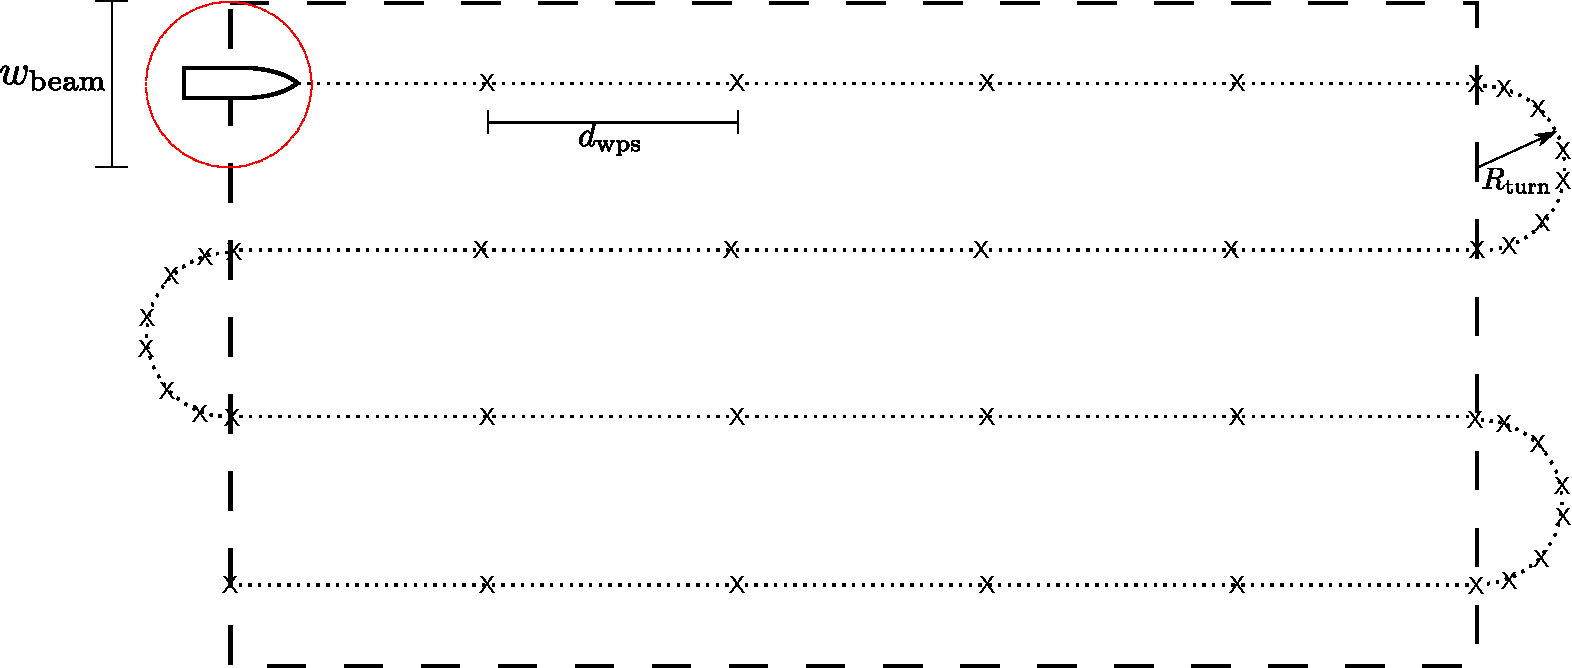
\includegraphics[width=1\textwidth]{figures/pathGen} 
  \caption{Area wanted to survey with waypoints}
  \label{fig:pathgen1}
\end{figure}   


